\chapter{Network Design}

\section{Topology}

The topology used for this lab assignment takes the form of a three router set-
up, simulating the infrastructure a typical Internet Service Provider (ISP)
might have. Using three routers as opposed to a one allows the ISP to make use
of additional technologies such as dynamic internal routing and iBGP in order
to create a fault-tolerant network. Using multiple devices results in increased
uptime as traffic can be routed via an alternate path should any outage occur
on any single device.

\begin{figure}[!ht]
    \caption{High-level Topology}
    \centering
    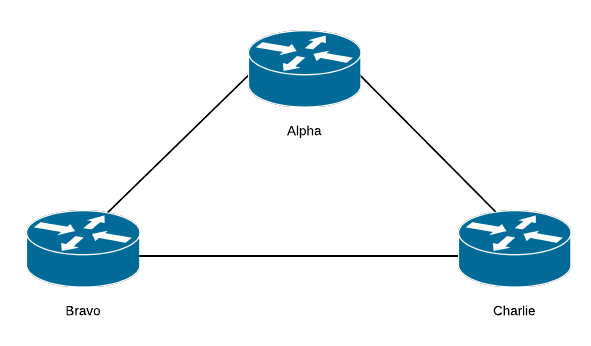
\includegraphics[width=0.8\textwidth]{images/networkTopology.png}
\end{figure}

\section{Address Allocation}
\subsection{IPv4}
For this lab exercise we represent the ISP BT and are assigned the IP block
\texttt{12.0.0.0/8} for our network. This address space provides us with 16.7
million addresses which can be allocated, of which we require only a small
fraction for our internal infrastructure. When allocating our address block we
took into account the issues that arose from the original allocation of
excessively large IPv4 network blocks to ISPs and Educational Institutions, we
decided it was best to be conservative in our allocations. With this in mind we
invented three classifications of network address, each defining the minimum
subnet size deemed necessary for its purpose. These are outlined in
Figure~\ref{figure:network-alloc-1}.

\begin{figure}[!ht]
    \caption{Classifications of Network Allocations}
    \label{figure:network-alloc-1}
    \centering
    \begin{tabular}{|c|c|p{5.5cm}|}

        \hline
        \textbf{Address Type} & \textbf{Subnet Mask} & \textbf{Justification} \\

        \hline
        Customer Segment & \texttt{/24} & These are allocated to downstream
        customers, who are given enough address space for 254 devices. In our network,
        laptops are used on these segments to test connectivity to customers. The size
        of this subnet also allows for easy identification of subnets to their location
        in the topology.\\

        \hline
        Point-to-point Links & \texttt{/30} & This is used for links that
        connect two routers, because for these links only two IP Addresses are required
        and a \texttt{/30} subnet mask is the smallest mask that will provide this.
        \textbf{Note:} The connection to our provider, AS 42, is an exception to this
        and uses a \texttt{/24} subnet mask as was provided by AS42.\\

        \hline
        Loopback Address & \texttt{/32} & Addresses used for the loopback
        interfaces on the routers, there is only a requirement for a single address and
        a \texttt{/32} mask produces this.\\

        \hline
    \end{tabular}
\end{figure}
In addition to the classification of subnets based on size, we used several IP
schemas to choose the IP values of our networks from our allocated block. This
allowed for quick identification of a network from its IP without referencing
our network diagrams. For example, customer segments connected to the Alpha
router have a 3rd octet value of 1, so it is immediately apparent that the IP
\texttt{12.0.1.0/24} is connected to Alpha.

These conventions were decided in advance of our network build-out and help us
diagnose issues with IP or interior routing configurations in a more intuitive
way. The exact schemas are outlined in Figure~\ref{figure:network-alloc-2}.

\begin{figure}[!ht]
    \caption{IP Schemas}
    \label{figure:network-alloc-2}
    \centering
    \begin{tabular}{|p{3cm}|p{3cm}|p{5cm}|}

        \hline
        \textbf{Schema} & \textbf{Classification} & \textbf{Identifying Feature} \\

        \hline
        \texttt{12.0.\#.0/24} & Customer Segment & The hash dictates the ISP
        router that this address space is connected to, 1 through 3 for Alpha, Bravo
        and Charlie. This would scale for up to 253 subnets in the Service Provider.\\
%why 253
        \hline
        \texttt{12.\#.0.0/30}, where $\#> 10$ & Peer Point-to-point Link &
        The hash in these networks dictates the assigned number of the group we connect
        to on these links. This enables us to quickly identify the group involved with
        any connectivity issues in BGP. For example, the link to group 3 uses the
        network \texttt{12.13.0.0/30}.\\

        \hline
        \texttt{12.0.0.\#/30} & Internal Point-to-point Link &
        The hash is a multiple of 4, starting from 0. This choice was arbitary.\\

        \hline
        \texttt{12.\#.\#.\#/32} & Loopback Address & The hash is
        the same value in all three octets of the address and dictates the router that
        this loopback is assigned to. For example, \texttt{12.3.3.3/32} is the loopback
        address of Charlie.\\

        \hline
    \end{tabular}
\end{figure}

\clearpage

\subsection{IPv6}
When allocating the IPv6 address-space we took a similar approach to that of
IPv4, aiming to allocate an appropriate sized address block to each segment of
the network. As such the classifications used are approximatly the same as
IPv4, with network segments being either a Customer Segment, Point-to-point
link or a Loopback. This is detailed in Figure~\ref{figure:network-alloc-3}.

\begin{figure}[!ht]
    \caption{Classifications of Network Allocations}
    \label{figure:network-alloc-3}
    \centering
    \begin{tabular}{|c|c|p{5.5cm}|}

        \hline \textbf{Address Type} & \textbf{Subnet Mask} & \textbf{Justification} \\

        \hline
        Customer Segment & \texttt{/36} & This address space is allocated for
        downstream connections to the ISPs customers, this currently has a large subnet
        mask which allows for it to be broken down into subnets containing the 48-bit
        Global Routing Prefix for customer networks.\\

        \hline
        Point-to-point Links & \texttt{/64} & These addresses
        are used for links that directly connect two routers, requiring two unique IP
        addresses. Reasons for the size of the subnet mask used are discussed below.\\

        \hline
        Loopback Address & \texttt{/128} & Addresses used for the loopback
        interfaces on the routers, there is only a requirement for a single address as
        was the case with IPv4. In IPv6 a \texttt{/128} mask produces this.\\

        \hline
    \end{tabular}
\end{figure}

The allocation of Customer Segments use a \texttt{/36} mask as a method of
breaking down our customer networks into a more manageable block of addresses.
The \texttt{/36} mask allows for BT to further break down their Customer
Segments into IPv6 blocks with a 48-bit Global Routing Prefix, which is a
unique ID for an IPv6 address which can be used identify both the ISP and the
customer.

In Figure~\ref{figure:network-alloc-3} it is obvious that applying a
\texttt{/64} mask allocates a considerable amount of addresses to a network
which would otherwise only require two unique addresses. The decision to use
this address was taken from RFC 4291, which dictates that ``For all unicast
addresses, except those that start with the binary value 000, Interface IDs are
required to be 64 bits long''~\cite{rfc4291}. In recent years there has been
discussions that the allocation of such a large amount of addresses is wasteful
and endorse the use of a \texttt{/127} mask. However this is not a standard and
for the purposes of this lab we have adhered to the RFC.
